%!TEX TS-program = lualatex

\documentclass[a4paper,12pt,table]{article}
\usepackage[utf8]{inputenc}
\usepackage[T1]{fontenc}

%!TEX TS-program = lualatex
\usepackage{tikz}
\usepackage{calc}
\usepackage{booktabs}
\usepackage[base]{babel}
\usepackage{hyperref}
\usepackage{graphicx}
\usepackage{wrapfig}
\usepackage{lipsum}
\usepackage[toc]{appendix}
\usepackage{xcolor}

% colors
\definecolor{color1}{HTML}{000060}
%\definecolor{color1}{HTML}{8C260F}
\definecolor{color2}{HTML}{333333}
\definecolor{lightgray}{gray}{0.9}

% fonts
\usepackage{fontspec}
\usepackage{unicode-math}
\defaultfontfeatures{Ligatures=TeX}
\setmainfont[Ligatures=TeX]{Candara}
%\setmathfont{XITS Math}
\newfontfamily\headingfont[]{Candara}
%%%

\usepackage{geometry}
\geometry{a4paper,
      hmargin=20mm,vmargin=20mm,
      head=0ex,foot=3ex}

\linespread{1.3}

\usepackage[hang]{caption}
\DeclareCaptionFormat{upper}{#1#2\uppercase{#3}\par}
\captionsetup{labelfont={bf,color=color2},textfont={normalsize,color=color2},format = upper,figurename=FIGURE,tablename=TABLE}

%%% fancy sections
\usepackage{titlesec}
%\titleformat{\chapter}{\headingfont\LARGE\bfseries\scshape\color{color1}}{\thechapter}{1em}{}[\titlerule]
\titleformat{\section}{\color{color1}\headingfont\Large\bfseries\uppercase}{\thesection}{1em}{}[\titlerule]
\titleformat{\subsection}{\color{color1}\headingfont\large\bfseries\uppercase}{\thesubsection}{1em}{}
\titleformat{\subsubsection}{\color{color1}\headingfont\bfseries\uppercase}{\thesubsubsection}{1em}{}
%%%

% head and foot
\usepackage{fancyhdr}
\pagestyle{fancy}
\lhead{}
\chead{}
\makeatletter
\rhead{\color{color2}\@date}
\makeatother
\newlength{\myheight}
\setlength{\headheight}{15pt}
\renewcommand\headrulewidth{0pt}
\renewcommand\footrulewidth{0pt}

%%% picture on cover page
\usepackage{eso-pic}
\newcommand\BackgroundPic{%
      \put(0,0){%
            \parbox[b][\paperheight]{\paperwidth}{%
                  \vfill
                  \centering
                  
\includegraphics[width=\paperwidth,height=\paperheight,%
                        keepaspectratio]{cover}%
                  \vfill
            }}}
%%%
% custom titlepage
\makeatletter
\renewcommand{\maketitle}{
      \thispagestyle{empty}
      \AddToShipoutPicture*{\BackgroundPic}
      \ClearShipoutPicture
      %
      \phantom{a}
      \vfill
      \phantom{a}\hfill
      \begin{tabular}[c]{@{}p{0.7\textwidth}@{}}
            \color{white}\headingfont\LARGE\@title  \\[1em]
            \color{white}\headingfont\Large\@author \\[2em]
      \end{tabular}
      %
      \clearpage
}
\makeatother
%%%


%%% fancy boxes
\usepackage{tcolorbox}
\usepackage{wrapfig}
\def\fullboxbegin{
      \bigskip
      \begin{tcolorbox}[colback=color1,colframe=color1,coltext=white,arc=0mm,boxrule=0pt]
            }
            \def\fullboxend{\end{tcolorbox}\medskip}
%
\def\leftboxbegin{
      \begin{wrapfigure}{l}{0.5\textwidth}
            \begin{tcolorbox}[colback=color1,colframe=color1,coltext=white,arc=0mm,boxrule=0pt]
                  }
                  \def\leftboxend{
            \end{tcolorbox}
      \end{wrapfigure}
}
%
\def\rightboxbegin{
      \begin{wrapfigure}{r}{0.5\textwidth}
            \begin{tcolorbox}[colback=color1,colframe=color1,coltext=white,arc=0mm,boxrule=0pt]
                  }
                  \def\rightboxend{
            \end{tcolorbox}
      \end{wrapfigure}
}
%
\newcounter{frames}
\def\frameboxbegin#1{
      \bigskip
      \refstepcounter{frames}
      \begin{tcolorbox}[colback=white,colframe=color1,arc=0mm,title={\MakeUppercase{\textbf{Frame \arabic{frames}}: #1}}]
            }
            \def\frameboxend{
      \end{tcolorbox}
}
%%%


%%%%%%%%%%%%%%%
% Title Page
\title{ADQ14 Hard X-Ray Monitor}
\author{Wojciech Walewski \newline DMCS}
\date{\today}
%%%%%%%%%%%%%%%

\begin{document}
\maketitle

\tableofcontents
\clearpage

\section{Introduction}

	\subsection{Document structure}
	This document describes the functionality of a firmware package developed for the ADQ14 digitizer.
	The solution implements a real time Pulse Height Analyzer for exponential pulses, 
	intended for use in Hard X-Ray Monitors. 
	The Pulse Height Analyzer firmware is built on top of the SPDevices ADQ14 DevKit.
	Initial chapters of this paper go over the digitizer board itself, 
	highlighting its features and limitations.
	The custom firmware solution is built on top of a development kit provided by SPDevices with ADQ14.
	\subsection{ADQ14}
	For information on the digitizer board itself refer to the 
	\href{https://www.spdevices.com/products/hardware/14-bit-digitizers/adq14}{manufacturers' website}.
	Specifically the 
	\href{https://www.spdevices.com/documents/datasheets/19-adq14-datasheet/file}{datasheet} 
	and the \href{https://www.spdevices.com/documents/user-guides/55-adq14-manual/file}{user manual}.
	
\newpage
\section{SPDevices DevKit}
	\begin{wrapfigure}[22]{r}{0.28\textwidth}
		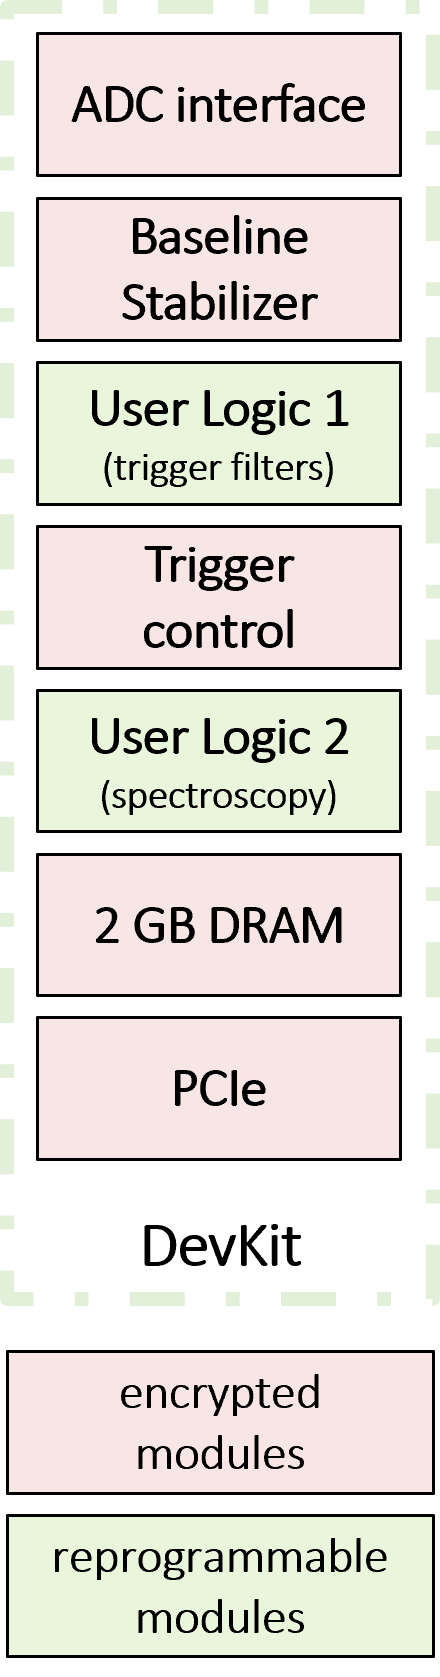
\includegraphics[width=0.25\textwidth]{img/devkit_ul.png}
		\caption{DevKit overview}\label{wrap-fig:devkit_ul}
	\end{wrapfigure}
	The custom spectroscopy firmware is built on top of a development kit provided with the digitizer board.
	The base system is referred to as the DevKit by the manufacturer. 
	A full documentation of the DevKit can be downloaded from the 
	\href{https://www.spdevices.com/documents/user-guides/24-adq14-development-kit}{manufacturer's website}.
	An offline copy is included with the firmware source code in the \verb|documentation| folder.
	\subsection{The concept of User Logic}
		The modules provided with the DevKit control the Analog Digital Converter, triggering,
		packeting, the DRAM data queue and the PCIe interface. The subsystems responsible for these
		parts of the pipeline are provided in the form of encrypted IP cores and cannot be modified.
		Two modifiable modules, referred to as User Logic 1 and 2, are exposed in between,
		enabling the use of entirely custom algorithms at two points in the data flow.
		User Logic 1 is placed right before the trigger control, enabling the use of
		detection or smoothing filters with the digitizer's level trigger feature.
		User Logic 2 allows for modifications being placed right before the individual consecutive
		samples are packed into records, assigned metadata and queued in the DRAM for transmission to the
		host computer. The DevKit structure, with the placement of the User Logic modules highlighted in gold,
		is shown in \autoref{wrap-fig:devkit_ul}. 
		Both modules are described in greater detail in the next chapters.
		\par
		\newpage
	\subsection{Samples in the FPGA}
		The digitizer's ADC is capable of sampling the signal at a rate up to 1 GS/s or 1 GHz.
		The FPGA is clocked at 250 MHz, resulting in a parallel design where each channel produces
		4 new consecutive samples for the FPGA on each clock cycle. The ADCs produce 14-bit samples.
		The raw signal is however subject to a digitial gain and shift.
		Two additional fractional bits are appended to the 14-bit samples before calculations.
		Two configurations are factored in the gain and shift calculations. 
		The board comes preconfigured with a factory calibration that is always applied. 
		A second configuration is made available to
		the users and can be freely modified from base values 
		to apply custom digital signal shift or change the gain.
	\subsection{Data flow in User Logic 1}
		After the digital gain and shift, the 16-bit samples are packed into a data bus 
		and made available at the User Logic 1 module. 
		This component is located before the level trigger. 
		By default the raw sample data is passed on to the triggering module unchanged. 
		If the device trigger mode is set to the level trigger,
		digital filters can be implemented in User Logic 1 to modify the trigger behaviour. 
		In initial testing a configurable moving average smoothing filter was placed in this module 
		to reduce the influence of noise.
		At one point a boxcar and a trapezoidal filters were successfully implemented for pulse detection.
		These filtering modules were created in an abstract manner 
		and can be combined to modify the level trigger
		behaviour to a desired shape and signal-to-noise ratio.
		\par
		The samples that are passed to the level trigger module can differ from those that are sent further
		down the processing pipeline, meaning that it is possible to trigger on appropriately filtered data,
		while still storing unmodified samples at the host PC. The current version of the firmware does not
		perform any filtering in this part of the firmware. All spectroscopy logic has been moved to User Logic 2,
		however the filter modules remain usable and can be reintroduced if the need appears.
	\subsection{Data flow in User Logic 2}\label{ssec:data_flow_in_user_logic_2}
		User Logic 2 deals with data that has passed through User Logic 1, 
		decimation and shifting to accomodate for pretrigger (horizontal shift). 
		User Logic 2 is responsible for tagging the start and end of a single acquisition window (record). 
		Further DevKit modules can then then pack and queue the records for transmission.
		User Logic 2 also inserts header data containing the metadata. 
		The record length is fixed by default and set in the control application on the host PC.
	\subsection{Data paths in the FPGA}
		\begin{figure}[!h]
			\centering
			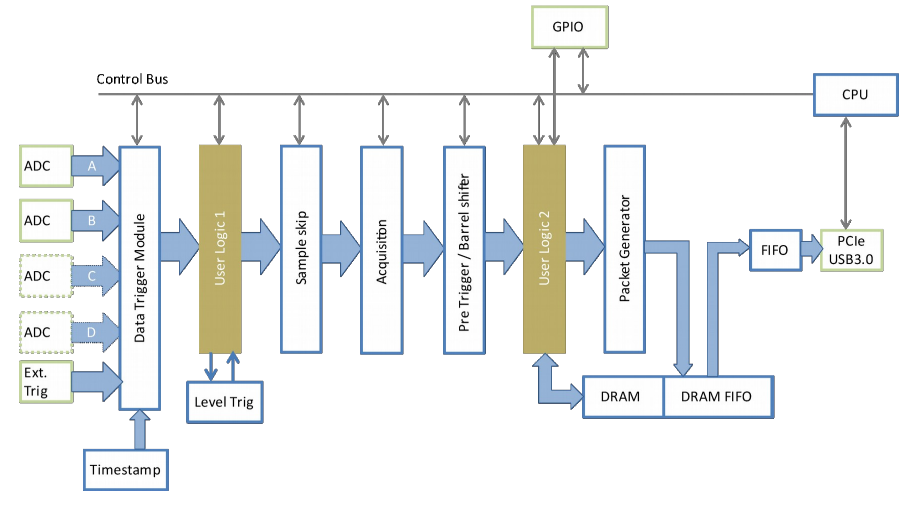
\includegraphics[width=\textwidth]{img/devkit_dataflow.png}
			\caption{Primary data flow in the FPGA}\label{fig:devkit_dataflow}
		\end{figure}
		\autoref{fig:devkit_dataflow} shows the primary data flow in the FPGA.
		Records built of the 16-bit samples, 
		together with the metadata are initially stored in the digitizer's internal DRAM. 
		This memory forms a FIFO queue, that is periodically transferred over to the host PC. 
		The ADQ14's RAM has a capacity of 2 GB. 
		With two bytes per sample up to a billion samples can be queued
		for data transfer before overflow leads to data loss. 
		With up to a billion samples being generated every second for every active channel, 
		this memory must be efficiently transferred.
		Two data paths exist within the firmware for exchanging data with the host PC.
		\subsubsection{DMA}
		After being packed in records and queued in the digitizer's DRAM, the acquired samples are sent
		using Direct Memory Access. This path makes it possible to write data directly to the host PC's RAM, 
		without the need of CPU involvment. Naturally, the host PC's RAM is not unlimited, 
		so the data must be processed (e.g. saved to a hard drive) at a rate comparable to the DMA transfers.
		DMA is a one-way path, so data can be transferred from the digitizer to the host PC,
		but not the other way around.
		Any data can be inserted in place of the samples for each channel to leverage the fast data path. 
		The custom Pulse Height Analyzer relies on this fact to periodically transfer computed spectras.
		\subsubsection{User Registers}
		A substantially slower two-way data path is available through the user registers 
		(top data bus on \autoref{fig:devkit_dataflow}). 
		Both User Logic modules implement a small individually addressable memory block, 
		that can be written to or read from by both the host PC and the FPGA. 
		The memory structure contains 32-bit integers. $2^{14}$ addressable words
		are available in User Logic 1, and $2^{19}$ in User Logic 2. 
		First 4 positions in both modules are reserved  for internal use by the DevKit 
		and cannot be modified in the custom firmware. The custom PHA firmware
		relies on User Registers primarily for transferring configuration settings to the FPGA.
		The current version of the firmware also enables spectra transfer 
		through this data path for testing purposes.
	\subsection{Bypassing User Logic}
		Both User Logic modules can be bypassed using the application available on the host PC. 
		When User Logic 1 is bypasssed, the incoming raw signal is fed directly to the board 
		trigger. Any filters placed there to improve the triggering performance will not work.
		When User Logic 2 is bypassed no signal data is transferred.
		Any logic placed there, like the spectroscope, will not output valid data.
		\begin{figure}[!h]
			\centering
			
\includegraphics[width=0.8\textwidth]{img/user_logic_1_bypass.png}
			\caption{Bypass in User Logic 1}\label{fig:user_logic_1_bypass}
		\end{figure}
\newpage
\section{Custom Firmware}
	The hardware spectroscopy solution consists of four primary subsystems:

	\begin{itemize}
		\item \hyperref[ssec:pulse_detection_module]{Pulse Detection and Timing Module}
		\item \hyperref[ssec:pulse_shaping_module]{Pulse Shaping Module}
		\item \hyperref[ssec:pulse_sampler]{Pulse Sampler}
		\item \hyperref[ssec:spectrum_storage_and_transfer]{Spectrum Storage and Transfer}
	\end{itemize}

	\begin{figure}[!h]
		\centering
		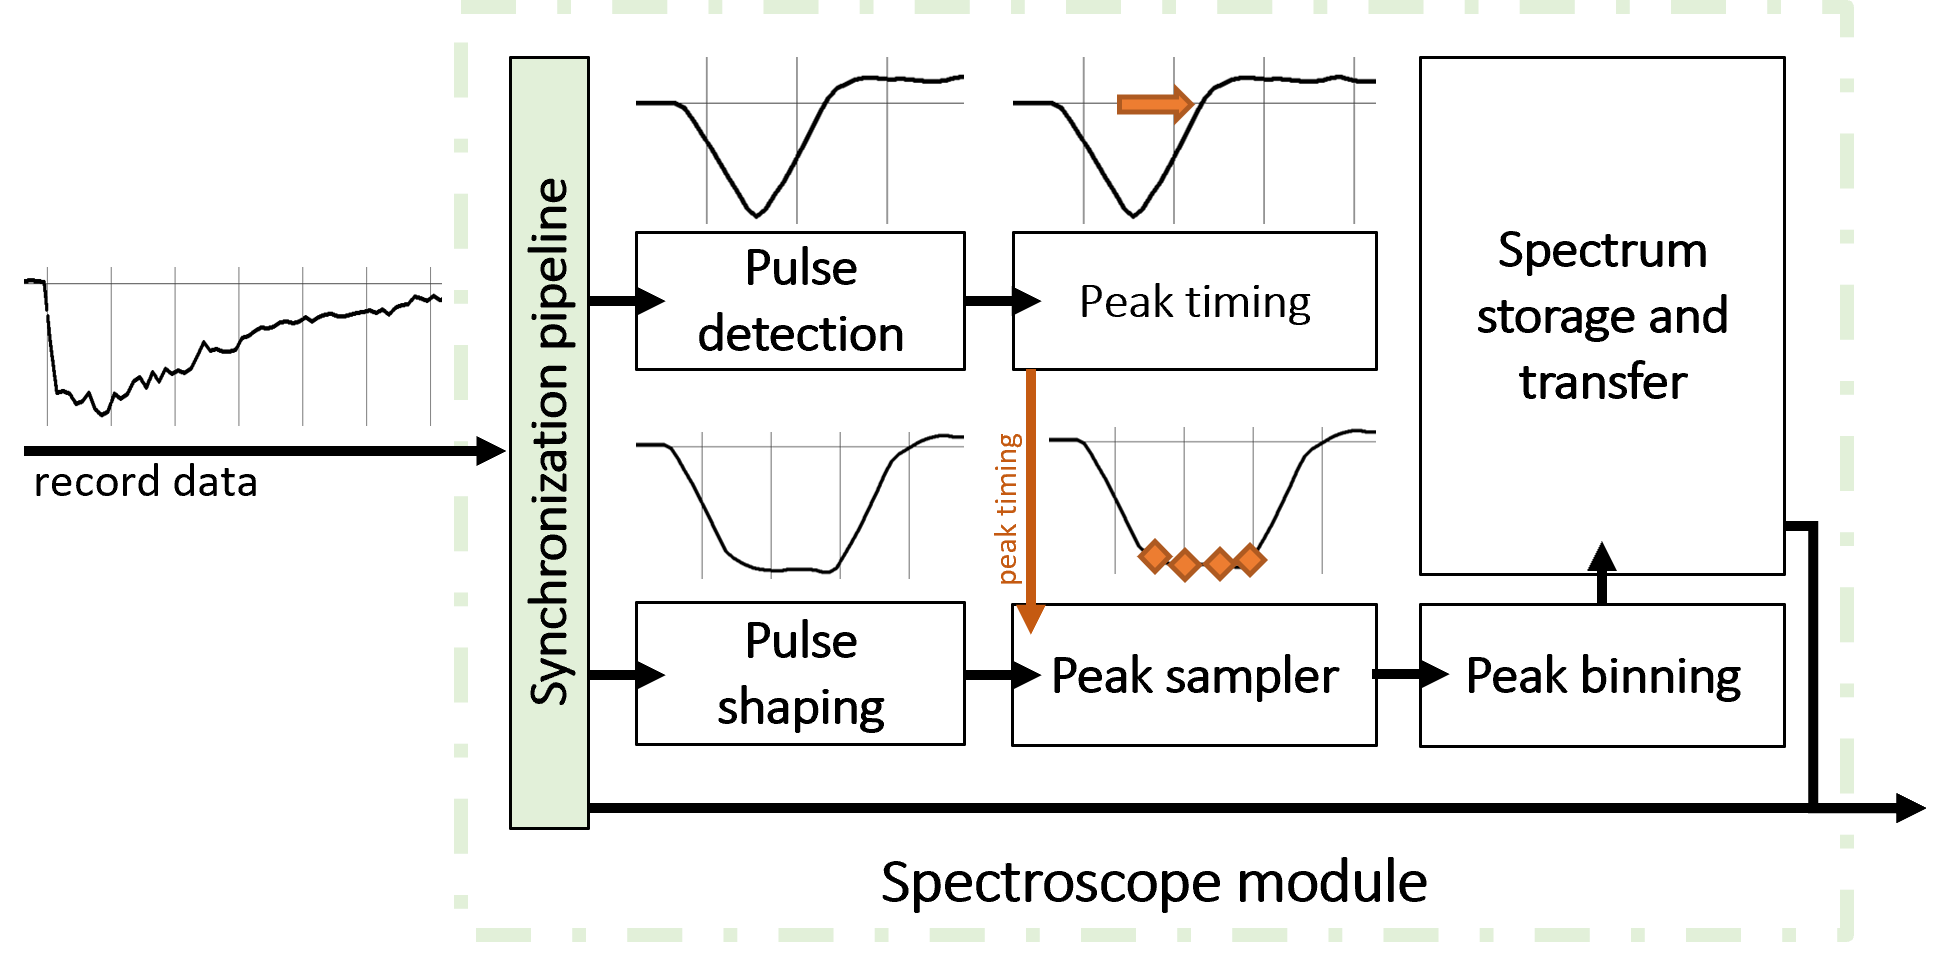
\includegraphics[width=0.9\textwidth]{img/user_logic_2_filters.png}
		\caption{Spectroscope module structure}\label{fig:user_logic_2_filters}
	\end{figure}

	The entire logic is located within the \hyperref[ssec:data_flow_in_user_logic_2]{User Logic 2} module. 
	\autoref{fig:user_logic_2_filters} presents the internal structure of the spectroscopy module and how 
	the different subcomponents operate. The incoming pulse record is passed to two submodules.
	A detection module combined with a timing one finds the horizontal position of the peak of a pulse.
	A tunable shaping filter modified the incoming pulses to reduce noise in the pulse height measurement.
	A sampler uses the timing information to measure an average peak height from the shaped pulse.
	Different signal filters require a different amount of clock cycles to process a single sample, 
	so they introduce a different delay to the signal. The timing filter must be synchronized to the shaping filter.
	This is achieved in a synchronization pipeline that delays the faster timing filter 
	by an appropriate number of clock cycles.
	\newpage
	\subsection{Pulse Detection and Timing Module}\label{ssec:pulse_detection_module}
		Pulse detection is done with the use of a zero crossing detector 
		applied to a digital bandpass filter in the form of a averaging derivative.	
		
		\begin{figure}[!ht]
			\centering
			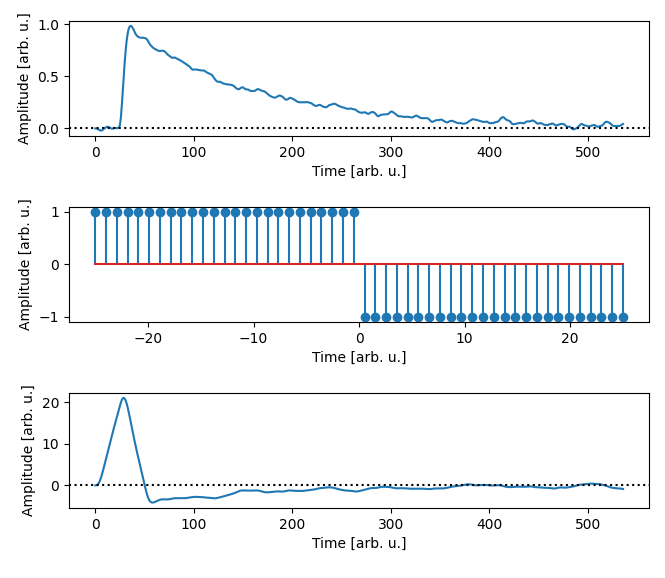
\includegraphics[width=0.60\textwidth]{img/boxcar_sim.png}
			\caption{Boxcar filter on a simulated unipolar exponential pulse}\label{fig:boxcar_sim}
		\end{figure}
		The incoming pulses are convolved with a boxcar filter. The result of such operation on 
		an exponential pulse, as well as an example boxcar transfer function are shown in \autoref{fig:boxcar_sim}.
		A unipolar pulse is transformed into a bipolar signal. The produced signal is a smoothed derivative, 
		so the point at the x-axis is crossed indicates the peak of a pulse.
		The averaging action present in the boxcar filter causes some delay, so for proper timing
		it must be accounted for in the timing module, that controls the sampling start.
		\newpage
		\begin{figure}[!h]
			\centering
			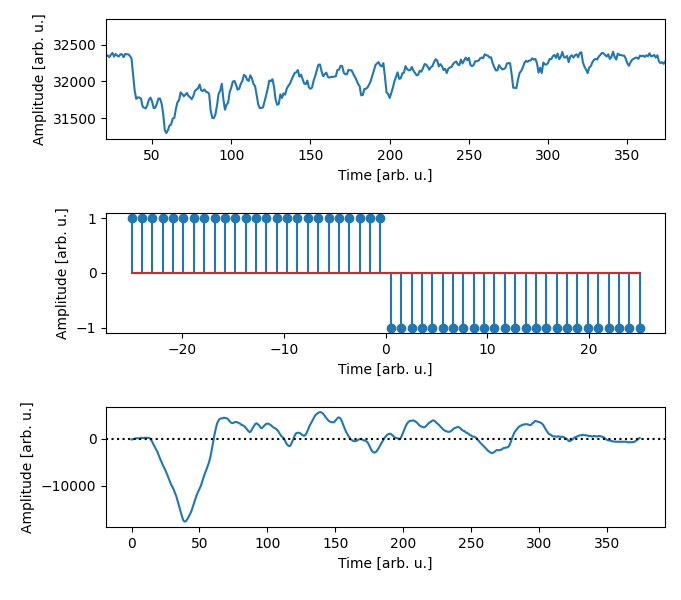
\includegraphics[width=0.60\textwidth]{img/boxcar_real.png}
			\caption{Boxcar filter on a real unipolar exponential pulse obtained from a radioactive source}\label{fig:boxcar_real}
		\end{figure}
		The boxcar filter is a versatile solution due to its relative simplicity. 
		\autoref{fig:boxcar_real} shows a boxcar filter being applied to a real exponential pulse
		obtained during tests with a radioactive $^{137}Cs$ sample. 
		The zero crossing point after the primary signal peak is preserved, 
		however the real signal is substantially less monotonic than simulated exponential pulses.
		To avoid false triggers, the Pulse Detection module applies thresholding.
		A threshold level is set using the software package 
		and transferred to the FPGA without a need for reprogramming. 
		When this value is crossed on the boxcar-filtered signal, 
		the detection module begins scanning for a zero crossing. 
		The timing data is sent to the \hyperref[ssec:pulse_sampler]{Pulse Sampler}
		and the module awaits another threshold crossing as shown in \autoref{fig:pulse_detection_thresholding}.
		\begin{figure}[!hb]
			\centering
			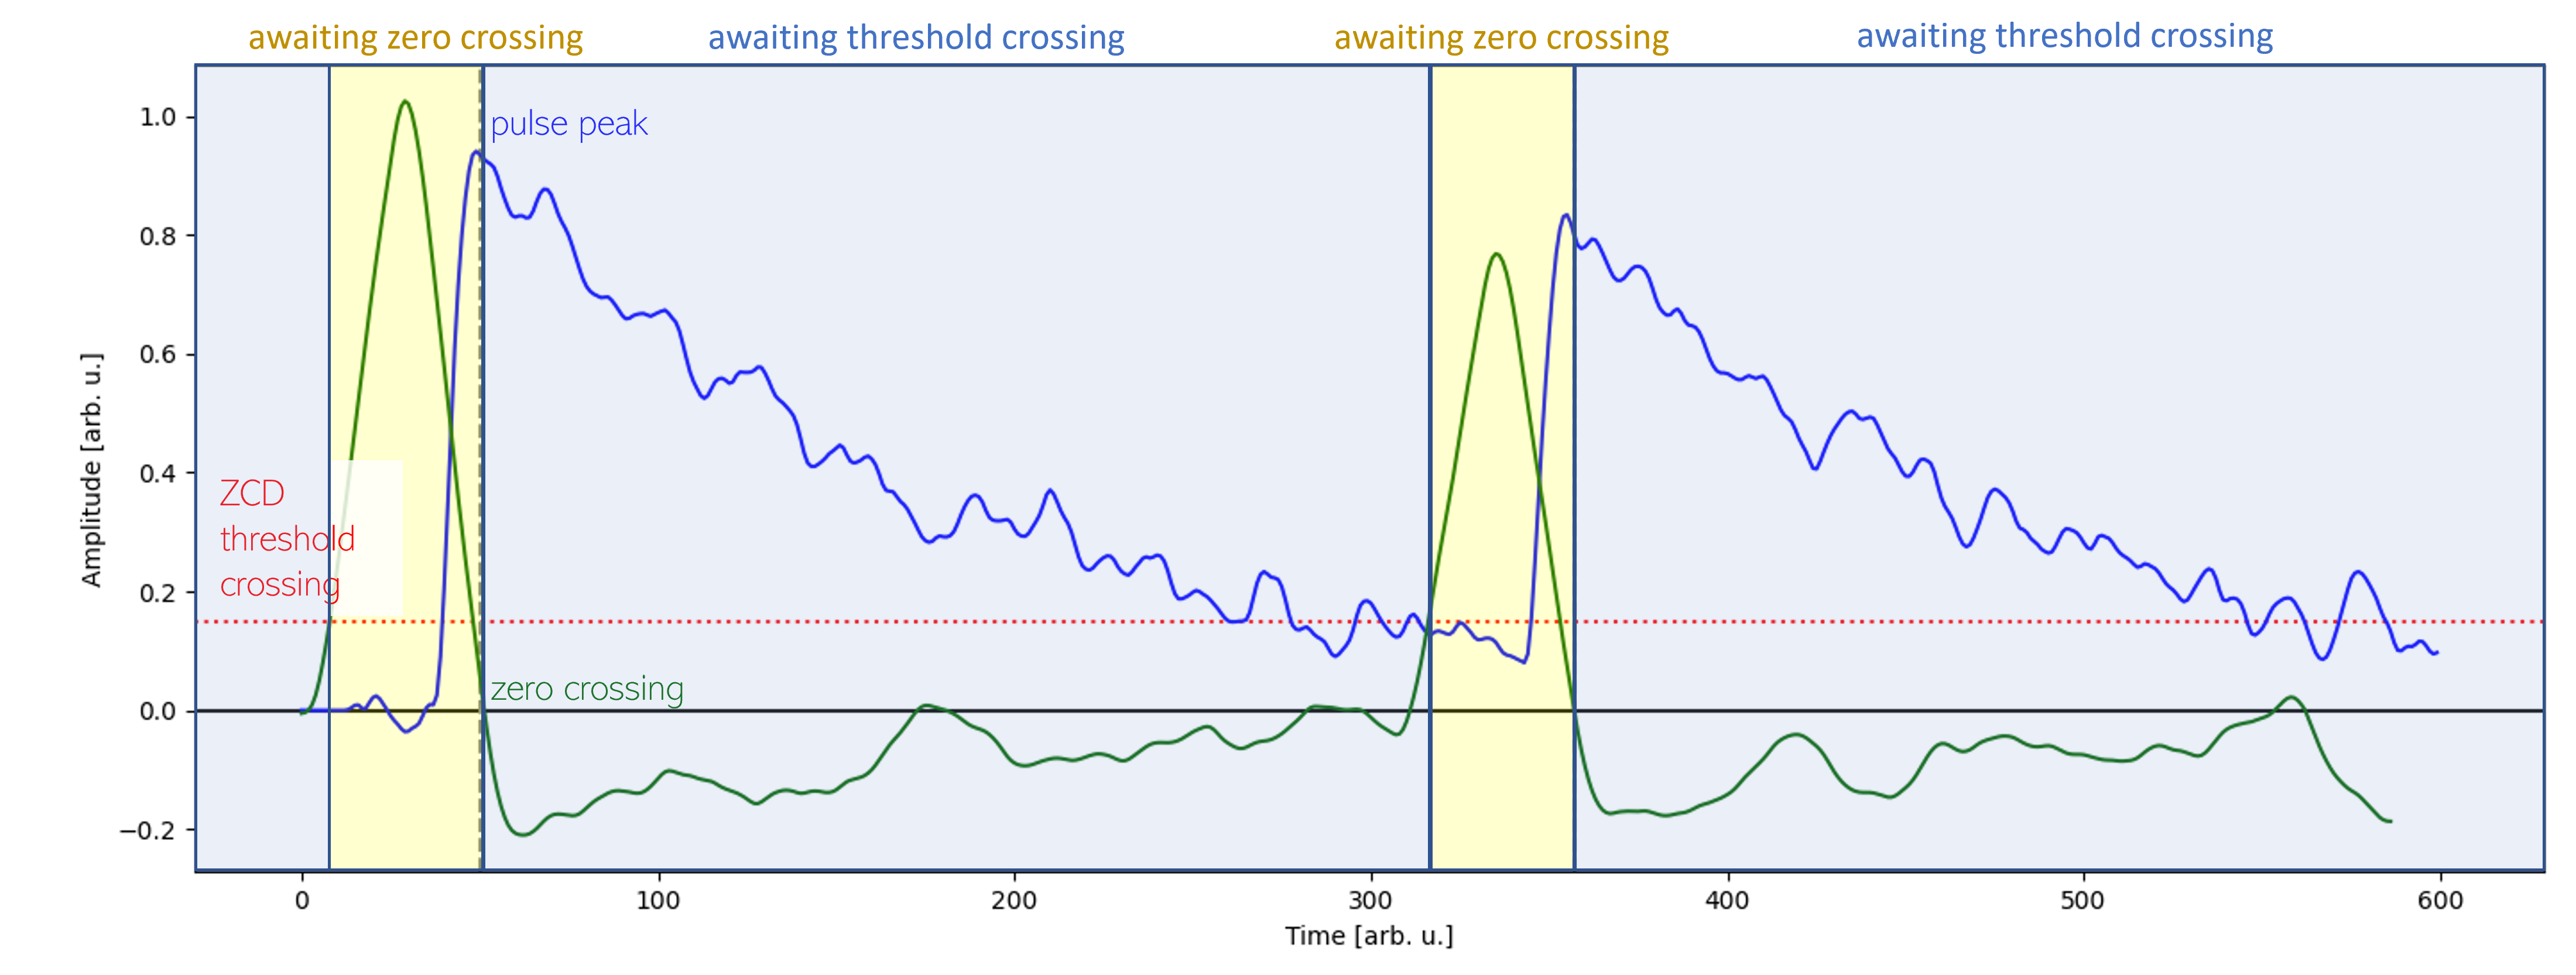
\includegraphics[width=\textwidth]{img/pulse_detection_internal.png}
			\caption{Pulse detection thresholding}\label{fig:pulse_detection_thresholding}
		\end{figure}
	\subsection{Pulse Shaping Module}\label{ssec:pulse_shaping_module}
		A trapezoidal filter is currently used to shape incoming pulses. 
		This type of filter offers a signal to noise ratio second only to a cusp filter.
		Generally it is not computationally expensive, however it introduces a large gain, 
		that must be attenuated at intermediate points 
		to remove the possibility of an integer overflow occuring in calculations.
		\autoref{fig:trapezoid_scheme} shows a block schematic of a trapezoid filter. 
		Three points which introduce a substantial amount of gain are highlighted.
		The gain is dependent on the parameters of the filters.
		\begin{figure}[!hb]
			\centering
			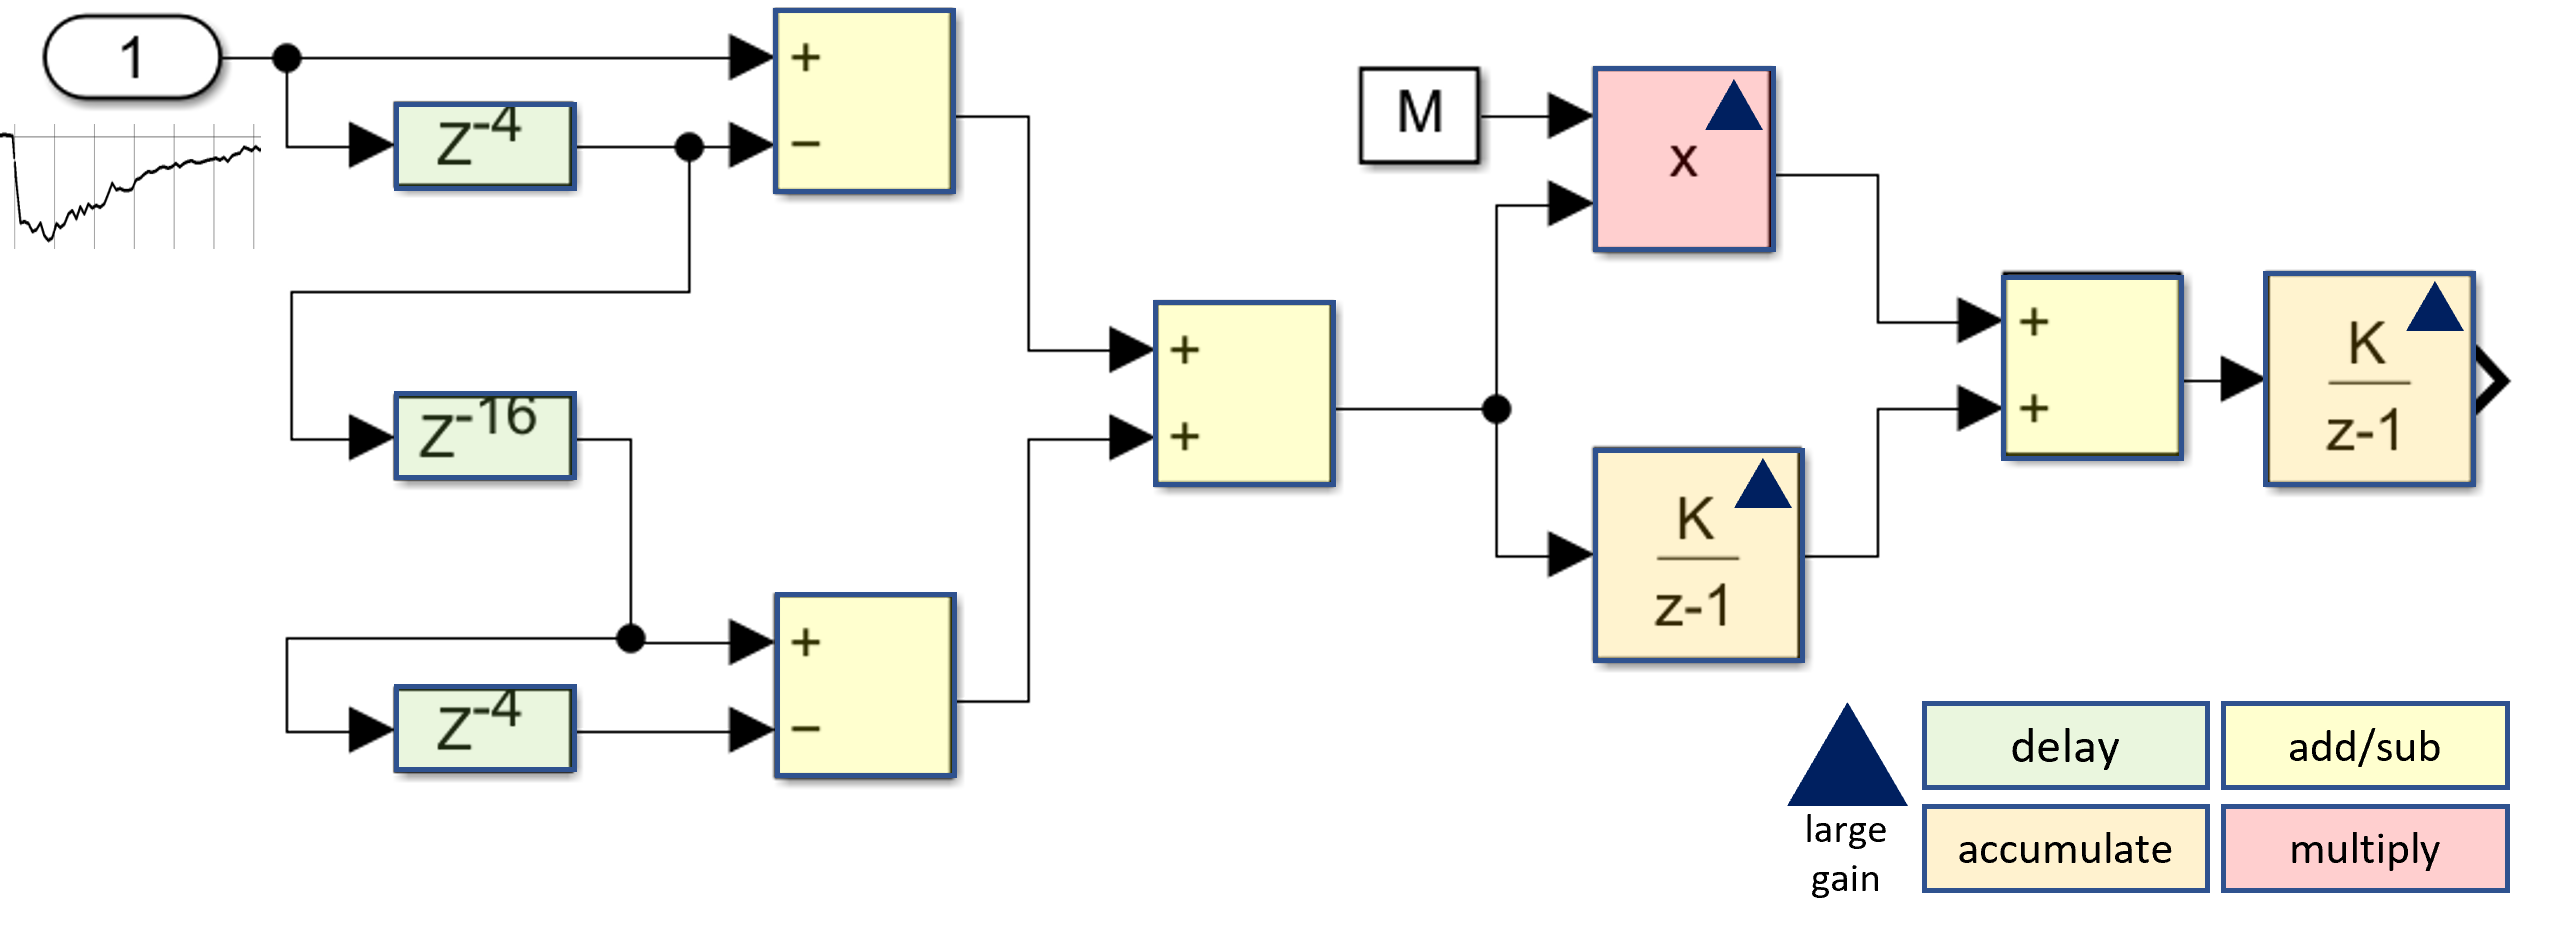
\includegraphics[width=\textwidth]{img/trapezoid_schematic.png}
			\caption{Trapezoid filter block scheme}\label{fig:trapezoid_scheme}
		\end{figure}
		Removing this gain requires division.
		Dividers can be implemented in firmware, however they result in complex circuitry,
		that in turn introduces substantial delay to the signals (20-30 clock cycles). 
		This increases the complexity of other components as they now have to include
		longer shit registers for synchornization.
		Where possible dividers were replaced with arithmetic shifters. 
	\subsection{Pulse Sampler}\label{ssec:pulse_sampler}
		Pulses shaped with the trapezoid filter form a flattop, 
		that linearly corresponds to the original pulse height.
		Due to noise in the system, sampling just the signal peaks
		would lead to subpar spectrum resolution. 
		The trapezoidal filter performs some averaging in accumulation stages,
		however the flattop region is never ideally horizontal.
		Multiple samples are taken at the flattop to improve the 
		result of pulse height measurement.
		\begin{figure}[!ht]
			\centering
			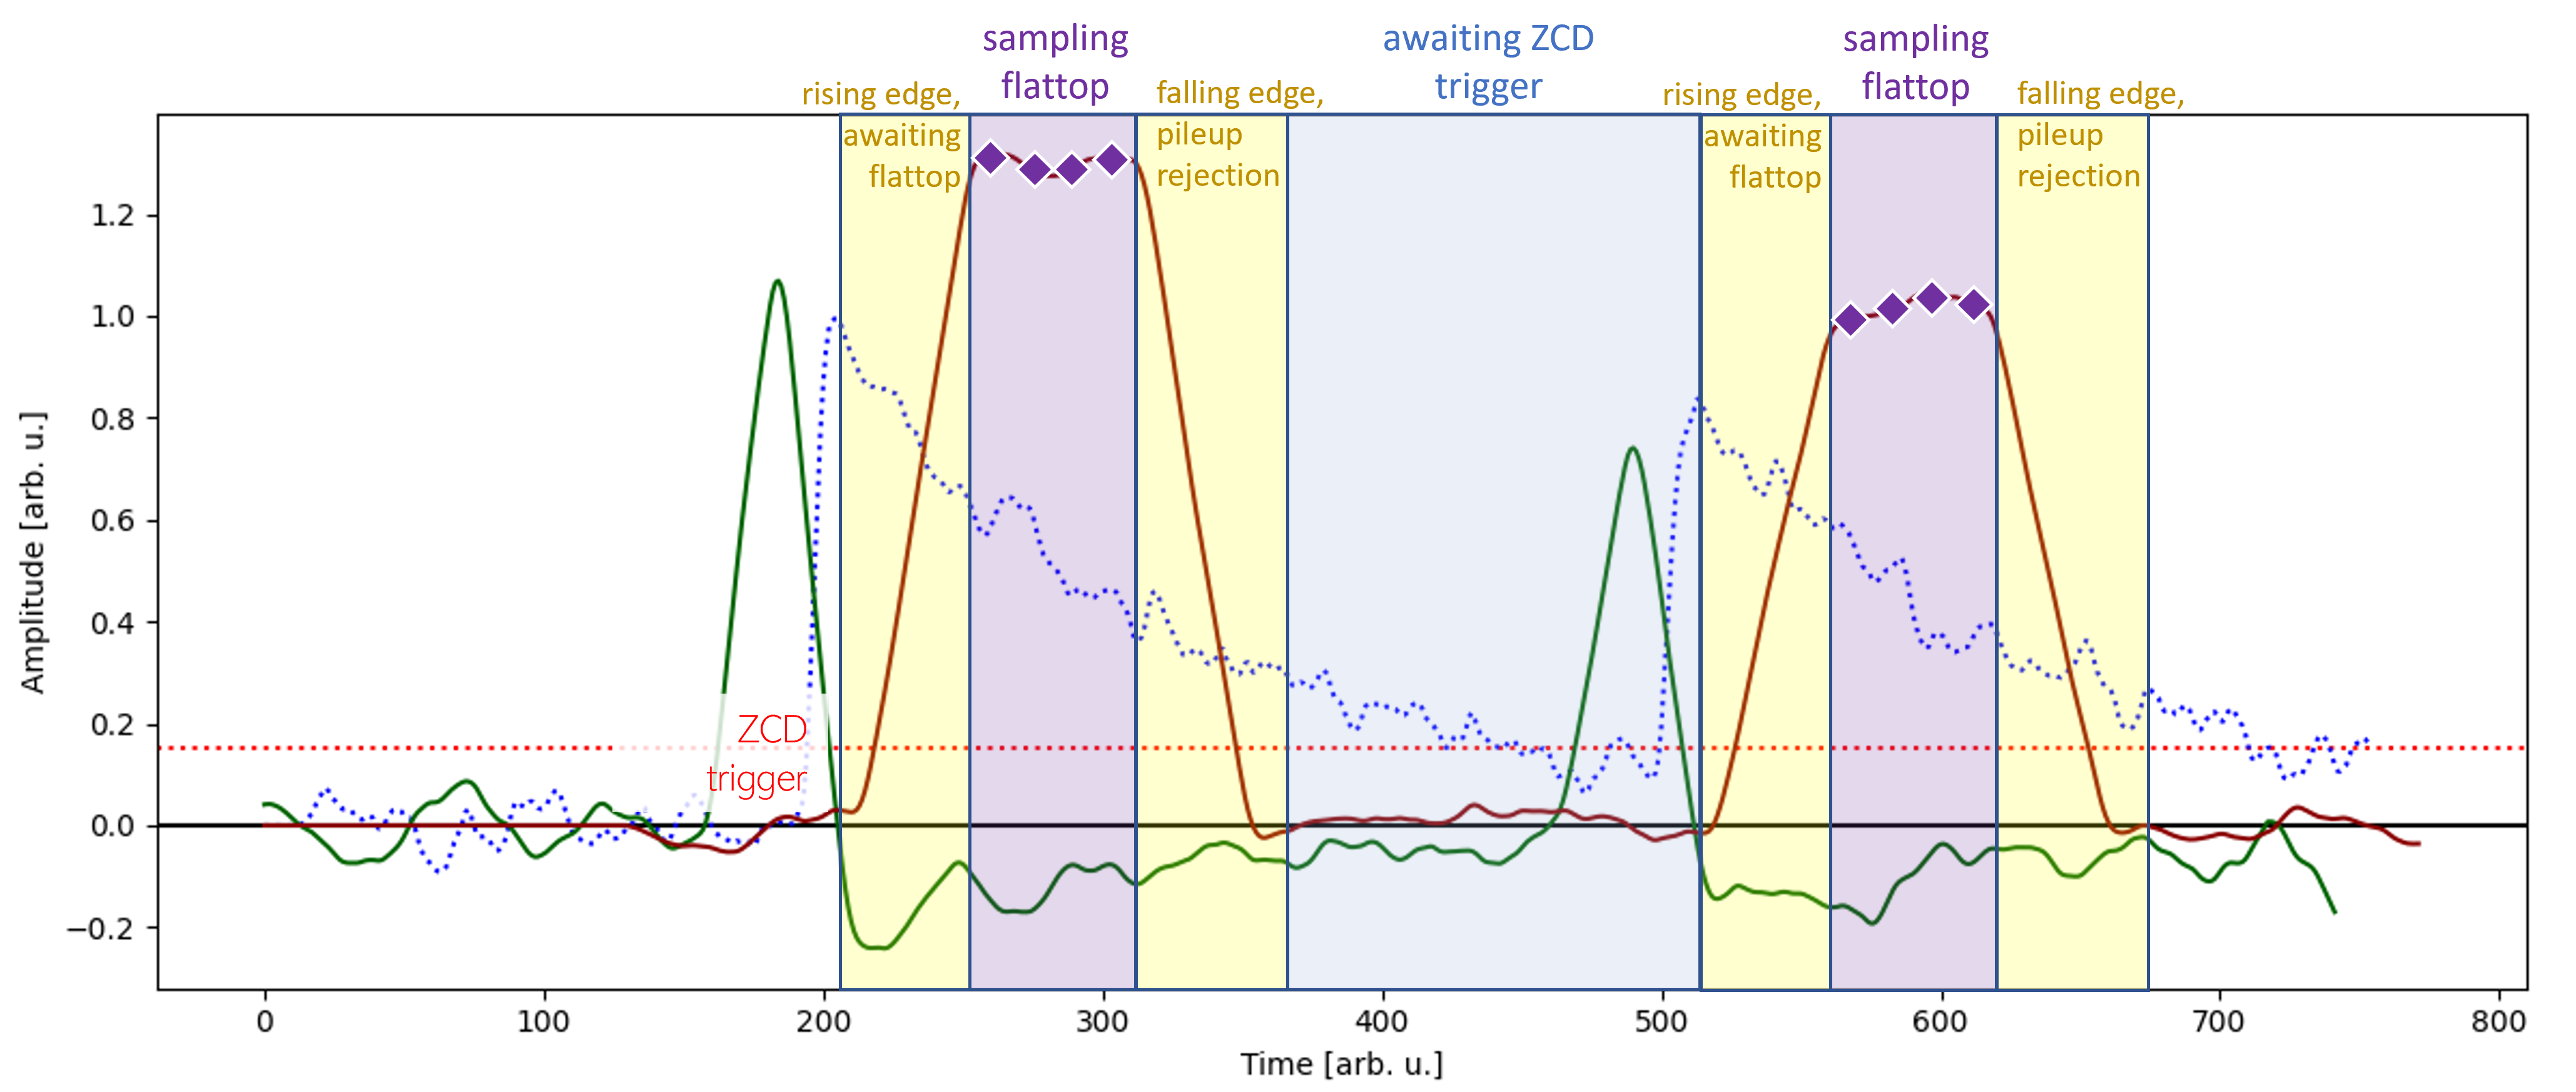
\includegraphics[width=\textwidth]{img/trapezoid_operation.png}
			\caption{Trapezoid filter block scheme}\label{fig:trapezoid_operation}
		\end{figure}
		As shown in \autoref{fig:trapezoid_operation}, the pulse sampler operates in states.
		This acts as a basic form of pile-up rejection. 
		A timing trigger from the \hyperref[ssec:pulse_detection_module]{Pulse Detection Module}
		causes the sampler to come into active state. 
		After watching the rising edge, upon reaching the flattop region, 
		an accumulator starts adding up samples.
		The duration of a flattop region is constant and defined by the trapezoid filter parameters,
		so the necessary division can be performed efficiently, 
		with a reliance on bit shifting or lookup tables.
		\newpage
	\subsection{Spectrum Storage and Transfer}\label{ssec:spectrum_storage_and_transfer}
		The measured pulse heights are binned into up to $2^{14}$ spectrum bins. 
		Without reprogramming the device the number of bins can be changed 
		into any power of $2$ lower than the maximum value.
		The measured pulse height is initially stored as a 16-bit unsigned integer. 
		The count of pulses in each bin is stored in an individually addressable
		dual port block RAM consiting of 32-bit words. 
		To translate the pulse height into a spectrum bin, and thus the RAM address, 
		$N$ most significant bits are taken from the pulse height, where $N$
		corresponds to the logarithm of the number of bins. 
		This is a very efficient design that does not require 
		divisors nor an array of comparataros, that would otherwise be necessary for binning.

\newpage
		\begin{figure}[!ht]
			\centering
			
\includegraphics[width=0.75\textwidth]{img/local_global_spectra.png}
			\caption{Local and global spectrum memory}\label{fig:local_global_spectra}
		\end{figure}
		As shown in \autoref{fig:local_global_spectra}, a total of 3 block RAMs are present in the design. 
		One, so called global BRAM, is entirely controlled through software.
		Appropriate bins are incremented as long as a flag in the FPGA registers is not unset.
		This acts primarily as a debuggin tool or in cases where a spectrum of an entire acquisition is necessary.
		Spectra are transferred from this BRAM with the use of user registers,
		so data should be read only when the board is not in an active acquisition.
		\par
		The other two BRAMs build windowed spectra. 
		The duration of the windows is configurable through the software package.
		In an example case of a 100 ms window, local BRAM A will be written to for 100 ms, 
		after which time the counting will immedietaly be taken over by local BRAM B. 
		During the next 100 ms window, local BRAM A will transfer its contents over the DMA channel 
		and reset all bin counts back to 0. This happens in approximately 25000 clock cycles,
		which translates to around 100 $\mu s$ of down time. 
		With the other local BRAM immedietaly taking over the counting, 
		this down time does not cause missed events, 
		as the active spectrum memory alternates with every window duration.
\newpage
\section{Using Custom Firmware}
	\subsection{Prerequisites}
		The DevKit firmware solution provided by SPDevices requires the use of Vivado 2015.2.
		The necessary version can be downloaded from 
		\href{https://www.xilinx.com/support/download/index.html/content/xilinx/en/downloadNav/vivado-design-tools/archive.html}{Vivado archives}.
		The custom software solution for controlling the digitizer and the custom firmware was built on top of
		ADQAPI library version [VERSION]. Using the ADQAPI in that version requires the following prerequisites to be installed:
		\begin{itemize}
			\item Lorem
			\item Ipsum
		\end{itemize}
		The ADQAPI library is distributed with the ADQ Digitizer board. 
	\subsection{QADQScope}
		The digitizer board, as well as the spectroscope firmware 
		are currently controlled from the same software application called QADQScope.
		The application allows users to start acquisitions with any 
		configuration available to the board. 
		\begin{figure}[!ht]
			\centering
			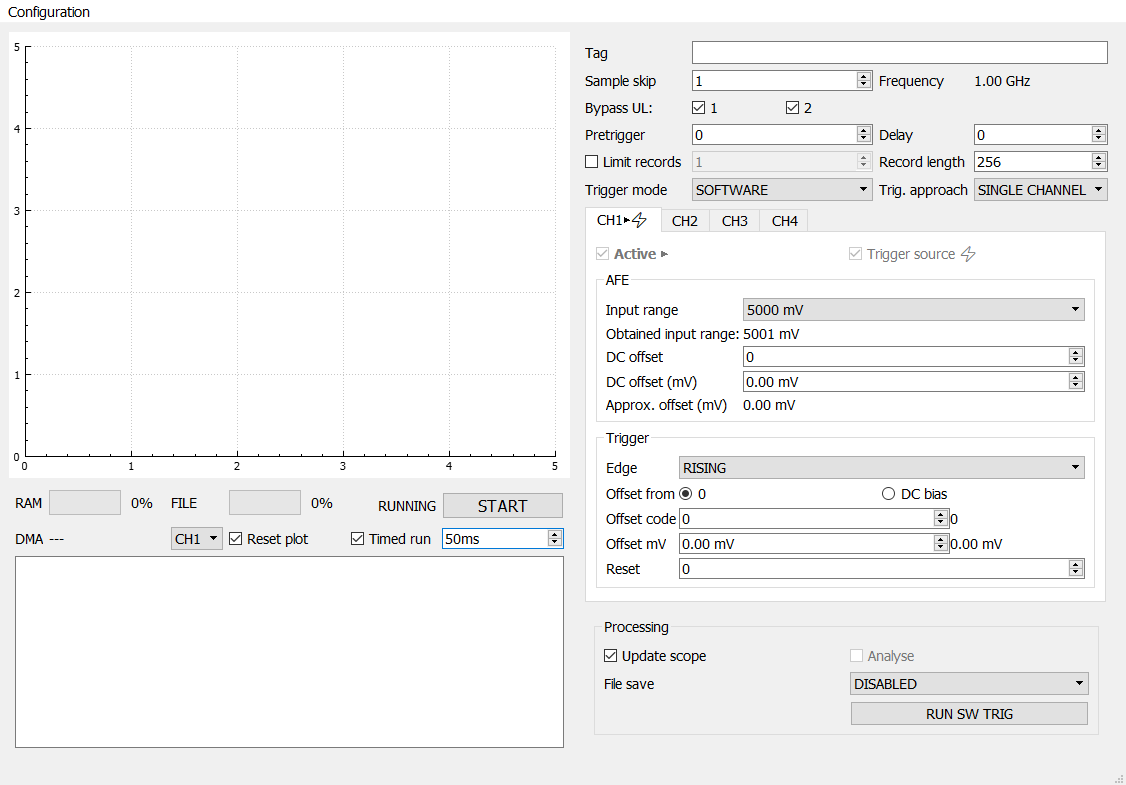
\includegraphics[width=\textwidth]{img/qtadqscope_main.png}
			\caption{Main window of QADQScope}\label{fig:qtadqscope_main}
		\end{figure}
		\autoref{fig:qtadqscope_main} shows the main window of QADQScope.
		This view is equipped with a plot window capable of displaying incoming
		records as they arrive to the host PC.
		Alternatively data can be saved to a hard drive. 
		While it is possible to simultanously save data and display it in real time,
		the plotting is significantly slower and will cause a bottleneck 
		in terms of processing speed.
		The primary view lets users change triggering configuration, 
		including record length and horizontal shift.
		To activate the custom firmware User Logic 2 must not be bypassed.
		\newpage
	\subsection{Spectrum Dialog}
		The primary Pulse Height Analyzer are available through a secondary dialog window 
		shown in \autoref{fig:qtadqscope_spectrum}.
		\begin{figure}[!ht]
			\centering
			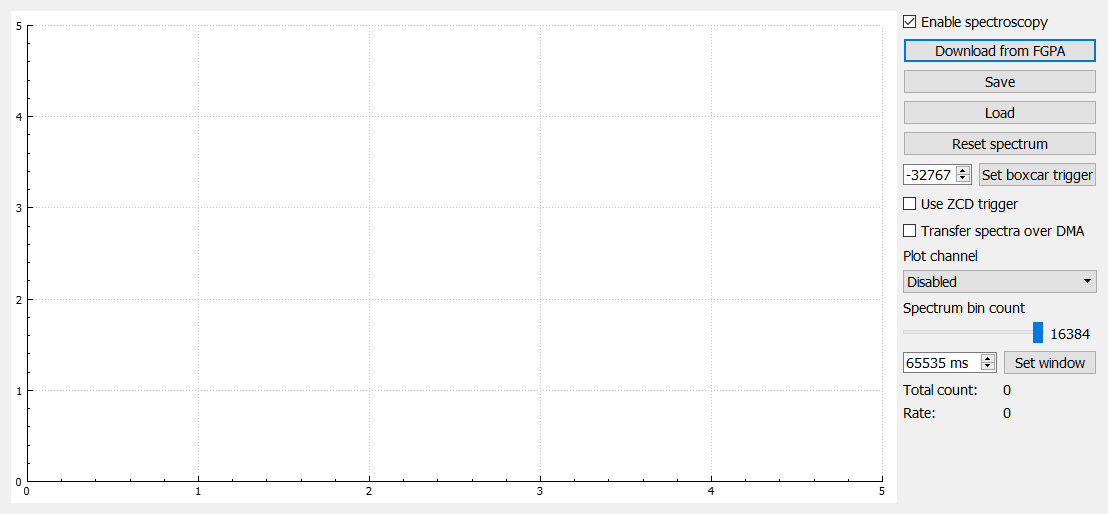
\includegraphics[width=\textwidth]{img/qtadqscope_spectrum.png}
			\caption{Spectrum dialog of QADQScope}\label{fig:qtadqscope_spectrum}
		\end{figure}
		To enable the spectroscope functionality the appropriate checkbox must be set.
		This enables the global spectrum counter. 
		The data from this memory is downloaded at user request 
		when the \verb|Download from FPGA button| is pressed.
		The \verb|Save| and \verb|Load| buttons allow for spectra to be written to or loaded from .csv files.
		To reset the counters in the global memory press the \verb|Reset spectrum| button.
		The boxcar trigger can be set to any value and functions as described in \autoref{ssec:pulse_detection_module}.
		The \verb|Transfer spectra over DMA| checkbox enables local memory
		with a window specified next to the \verb|Set window| button.
		The transferred windowed spectra can be displayed in real time on the plot available in this dialog window.
		Changing the bin count is achieved via the slider. 
		After every change to the bin count it is necessary to reset the global spectrum.
		Otherwise the counts will not be reset automatically
		and the new data will be superposed with the previously existing one.
\newpage


\end{document}
